\documentclass[
	% -- opções da classe memoir --
	12pt,				% tamanho da fonte
	openright,			% capítulos começam em pág ímpar (insere página vazia caso preciso)
	%twoside,			% para impressão em recto e verso. Oposto a oneside
	oneside,      % para impressão direta das páginas. Oposto a twoside
	a4paper,			% tamanho do papel.
	% -- opções da classe abntex2 --
	%chapter=TITLE,		% títulos de capítulos convertidos em letras maiúsculas
	%section=TITLE,		% títulos de seções convertidos em letras maiúsculas
	%subsection=TITLE,	% títulos de subseções convertidos em letras maiúsculas
	%subsubsection=TITLE,% títulos de subsubseções convertidos em letras maiúsculas
	% -- opções do pacote babel --
	english,			% idioma adicional para hifenização
	french,				% idioma adicional para hifenização
	spanish,			% idioma adicional para hifenização
	brazil,				% o último idioma é o principal do documento
	]{abntex2}\usepackage[]{graphicx}\usepackage[table]{xcolor}
% maxwidth is the original width if it is less than linewidth
% otherwise use linewidth (to make sure the graphics do not exceed the margin)
\makeatletter
\def\maxwidth{ %
  \ifdim\Gin@nat@width>\linewidth
    \linewidth
  \else
    \Gin@nat@width
  \fi
}
\makeatother

\definecolor{fgcolor}{rgb}{0.345, 0.345, 0.345}
\newcommand{\hlnum}[1]{\textcolor[rgb]{0.686,0.059,0.569}{#1}}%
\newcommand{\hlstr}[1]{\textcolor[rgb]{0.192,0.494,0.8}{#1}}%
\newcommand{\hlcom}[1]{\textcolor[rgb]{0.678,0.584,0.686}{\textit{#1}}}%
\newcommand{\hlopt}[1]{\textcolor[rgb]{0,0,0}{#1}}%
\newcommand{\hlstd}[1]{\textcolor[rgb]{0.345,0.345,0.345}{#1}}%
\newcommand{\hlkwa}[1]{\textcolor[rgb]{0.161,0.373,0.58}{\textbf{#1}}}%
\newcommand{\hlkwb}[1]{\textcolor[rgb]{0.69,0.353,0.396}{#1}}%
\newcommand{\hlkwc}[1]{\textcolor[rgb]{0.333,0.667,0.333}{#1}}%
\newcommand{\hlkwd}[1]{\textcolor[rgb]{0.737,0.353,0.396}{\textbf{#1}}}%
\let\hlipl\hlkwb

\usepackage{framed}
\makeatletter
\newenvironment{kframe}{%
 \def\at@end@of@kframe{}%
 \ifinner\ifhmode%
  \def\at@end@of@kframe{\end{minipage}}%
  \begin{minipage}{\columnwidth}%
 \fi\fi%
 \def\FrameCommand##1{\hskip\@totalleftmargin \hskip-\fboxsep
 \colorbox{shadecolor}{##1}\hskip-\fboxsep
     % There is no \\@totalrightmargin, so:
     \hskip-\linewidth \hskip-\@totalleftmargin \hskip\columnwidth}%
 \MakeFramed {\advance\hsize-\width
   \@totalleftmargin\z@ \linewidth\hsize
   \@setminipage}}%
 {\par\unskip\endMakeFramed%
 \at@end@of@kframe}
\makeatother

\definecolor{shadecolor}{rgb}{.97, .97, .97}
\definecolor{messagecolor}{rgb}{0, 0, 0}
\definecolor{warningcolor}{rgb}{1, 0, 1}
\definecolor{errorcolor}{rgb}{1, 0, 0}
\newenvironment{knitrout}{}{} % an empty environment to be redefined in TeX

\usepackage{alltt}

% ---
% PACOTES
% ---

% ---
% Pacotes fundamentais
% ---
\usepackage{lmodern}			% Usa a fonte Latin Modern
\usepackage[T1]{fontenc}		% Selecao de codigos de fonte.
\usepackage[utf8]{inputenc}		% Codificacao do documento (conversão automática dos acentos)
\usepackage{indentfirst}		% Indenta o primeiro parágrafo de cada seção.
\usepackage{color}				% Controle das cores
\usepackage{graphicx}			% Inclusão de gráficos
\usepackage{microtype} 			% para melhorias de justificação
% ---
\usepackage{booktabs}
\usepackage[table]{xcolor}
\usepackage{amssymb}
\usepackage{amsthm}
\usepackage{float}
\usepackage{here}

\usepackage{amsmath}
\usepackage{epstopdf}

% ---
\theoremstyle{definition}
\newtheorem{definition}{Definição}[section]

\theoremstyle{remark}
\newtheorem*{remark}{Remark}
% ---
% Pacotes adicionais, usados apenas no âmbito do Modelo Canônico do abnteX2
% ---
%\usepackage{lipsum}				% para geração de dummy text
% ---

% ---
% Pacotes de citações
% ---
\usepackage[brazilian,hyperpageref]{backref}	 % Paginas com as citações na bibl
\usepackage[alf]{abntex2cite}	% Citações padrão ABNT

% ---
% CONFIGURAÇÕES DE PACOTES
% ---

% ---
% Configurações do pacote backref
% Usado sem a opção hyperpageref de backref
\renewcommand{\backrefpagesname}{Citado na(s) página(s):~}
% Texto padrão antes do número das páginas
\renewcommand{\backref}{}
% Define os textos da citação
\renewcommand*{\backrefalt}[4]{
	\ifcase #1 %
		Nenhuma citação no texto.%
	\or
		Citado na página #2.%
	\else
		Citado #1 vezes nas páginas #2.%
	\fi}%
% ---

% ---
% Informações de dados para CAPA e FOLHA DE ROSTO
% ---
\titulo{Análise de Séries Temporais: Aplicação do modelo ARIMA para previsão do Preço da Soja}
\autor{DOUGLAS VINÍCIUS GONÇALVES ARAÚJO}
\local{JI-PARANÁ}
\data{2022}
\instituicao{%
  UNIVERSIDADE FEDERAL DE RONDÔNIA -- UNIR
  \par
  DEPARTAMENTO DE MATEMÁTICA E ESTATÍSTICA
  \par
  RELATÓRIO DE PESQUISA}
\tipotrabalho{Tese (Doutorado)}
% O preambulo deve conter o tipo do trabalho, o objetivo,
% o nome da instituição e a área de concentração
\preambulo{Relatório de Pesquisa na disciplina de Séries Temporais, do curso de Bacharel em Estatística da Universidade Federal de Rondônia, \textit{campus} Ji-Paraná, como requisito de avaliação.}
% ---

% ---
% Configurações de aparência do PDF final

% alterando o aspecto da cor azul
\definecolor{blue}{RGB}{41,5,195}

% informações do PDF
\makeatletter
\hypersetup{
     	%pagebackref=true,
		pdftitle={\@title},
		pdfauthor={\@author},
    	pdfsubject={\imprimirpreambulo},
	    pdfcreator={LaTeX with abnTeX2},
		pdfkeywords={abnt}{latex}{abntex}{abntex2}{projeto de pesquisa},
		colorlinks=true,       		% false: boxed links; true: colored links
    	linkcolor=blue,          	% color of internal links
    	citecolor=blue,        		% color of links to bibliography
    	filecolor=magenta,      		% color of file links
		urlcolor=blue,
		bookmarksdepth=4
}
\makeatother
% ---

% ---
% Espaçamentos entre linhas e parágrafos
% ---

% O tamanho do parágrafo é dado por:
\setlength{\parindent}{1.3cm}

% Controle do espaçamento entre um parágrafo e outro:
\setlength{\parskip}{0.2cm}  % tente também \onelineskip

% ---
% compila o indice
% ---
\makeindex
% ---

% ----
% Início do documento
% ----
\IfFileExists{upquote.sty}{\usepackage{upquote}}{}
\begin{document}

% Seleciona o idioma do documento (conforme pacotes do babel)
%\selectlanguage{english}
\selectlanguage{brazil}

% Retira espaço extra obsoleto entre as frases.
\frenchspacing

% ----------------------------------------------------------
% ELEMENTOS PRÉ-TEXTUAIS
% ----------------------------------------------------------
% \pretextual

% ---
% Capa
% ---
\imprimircapa
% ---

% ---
% Folha de rosto
% ---
\imprimirfolhaderosto
% ---
\clearpage
% ---
% NOTA DA ABNT NBR 15287:2011, p. 4:
%  ``Se exigido pela entidade, apresentar os dados curriculares do autor em
%     folha ou página distinta após a folha de rosto.''
% ---
% Epígrafe

\begin{epigrafe} 
  \vspace*{\fill} 
  \begin{flushright} 
  \textit{"Os livros servem para nos lembrar quanto somos estúpidos e tolos. 
      \\ São o guarda pretoriano de César, cochichando enquanto o desfile ruge 
      \\ pela avenida: – Lembre-se, César, tu és mortal. A maioria de nós não 
      \\ pode sair correndo por aí, falar com todo mundo, conhecer todas as 
      \\ cidades do mundo, não temos tempo, dinheiro ou tantos amigos assim. 
      \\ As coisas que você está procurando, Montag, estão no mundo, mas a 
      \\ única possibilidade que o sujeito comum terá de ver noventa e nove 
      \\ por cento delas está num livro". 
      \\ - Fahrenheit 451 de Ray Douglas Bradbury} 
  \end{flushright} 
\end{epigrafe}
% ---
% --- resumo em português--
\begin{resumo} 
O objetivo deste trabalho tem como propor a análise do comportamento do preço médio mensal da saca de 60kg (R\$/sc), bem como a previsão aplicada a modelagem ARIMA (Modelo Médio Integrado Auto-Regressivo) da \textit{commodities} de soja no Brasil. Os dados de séries foram coletados no site CEPEA (Centro de Estudos Avançados em Economia Aplicada) da metodologia soja CEPEA/ESALQ - PARANÁ, entre os intervalos de agosto de 1997 a outubro de 2022. Empregamos a metodoliga Box-Jenkins (1976) com o designo de encontrar o melhor ajuste do modelo de série temporal com base histórica dos preços. Ademais, foi utilizado uma função automatizada do pacote "forecast" do Sofware R para obter o modelo ideal para série. Assim, o modelo \textbf{ARIMA}(1,1,0)(2,0,0) foi o melhor para prever o preço médio mensal de soja. Os resultados ilustram um tendência crescente nos preços e na decomposição da série viu-se que há sazonalidade. Assim, este estudo pode fornecer uma abordagem como método de apoio à tomada de decisão para formular a previsão de preço da soja para o mercado brasileiro.
  \vspace{\onelineskip} 
  \noindent
  
  \textbf{Palavras-chaves}: Séries Temporais, Modelo ARIMA, Preços da Soja.
\end{resumo}

% ---
% inserir lista de ilustrações
% ---
\pdfbookmark[0]{\listfigurename}{lof}
\listoffigures*
\cleardoublepage
% ---

% ---
% inserir lista de tabelas
% ---
\pdfbookmark[0]{\listtablename}{lot}
\listoftables*
\cleardoublepage
% ---

% ---
% inserir lista de abreviaturas e siglas
% ---
%\begin{siglas}
%  \item [EMBRAPA] Empresa Brasileira de Pesquisa Agropecuária
%  \item [CEPEA]   Centro de Estudos Avançados em Economia Aplicada
%  \item [CONAB  ] Companhia Nacional de Abastecimento
%  \item [v.a.   ] Variável aleatória
%  \item [fdp    ] Função densidade de probabilidade
%\end{siglas}
% ---

% ---
% inserir lista de símbolos
% ---
%\begin{simbolos}
%  \item[$ \Gamma $] Letra grega Gama
%  \item[$ \Lambda $] Lambda
%  \item[$ \zeta $] Letra grega minúscula zeta
%  \item[$ \in $] Pertence
  
%\end{simbolos}
% ---

% ---
% inserir o sumario
% ---
\pdfbookmark[0]{\contentsname}{toc}
\tableofcontents*
\cleardoublepage
% ---

% ----------------------------------------------------------
% ELEMENTOS TEXTUAIS
% ----------------------------------------------------------
\textual

% ----------------------------------------------------------
% Introdução
% ----------------------------------------------------------
\chapter[Introdução]{Introdução}
%\addcontentsline{toc}{chapter}{INTRODUÇÃO}



A soja derivou na costa leste da Ásia, nas aproximidades do rio Yangtse na China. Antigamente a soja eram plantas rasteiras, bem distinta de hoje que cultivamos que foram modificadas e melhoradas pelo chineses. Apesar de ser conhecida e consumida pela civilização oriental por milhares de anos, ocorreu a sua introdução na Europa no final do século XV. 

No Brasil, na década de 60, dois fatores internos que fizeram a produção de 
soja expandir, fatores estes que influênciaram o cenário mundial da produção de grãos: \textit{i)} com o esforço da produção de suínos e aves assim gerava demanda pelo farelo de soja, já erá uma necessidade estratégica; \textit{ii)} na década de 70 houve a explosão 
do preço da soja no mercado mundial e os agricultores e o governo beneficiavam de um 
vantagem competitiva em relação de outros países, pois o escoamente da safra brasileira ocorre na entressafra americana, quando os preços atingem as maiores cotações, em conformidade com \cite{embrapa2022}.


A produção de soja avançou significativamente no mundo nestes últimos 20 anos, com taxas 
de crescimento de $3,7\%$ ao ano. Os três maiores produtores de soja mundial, juntos, respondem por mais de $80\%$ da produção, que são Brasil, Estados Unidos (EUA) e Argentina. E destes, o país que mais apresentou taxa de crescimento da produção nessas últimas décadas é o Brasil, com aumento de $5,9\%$ a. a., superior entre os seus concorrentes (EUA avançou $2,7\%$ a. a. e a Argentina $1,6\%$ a. a.), segundo \cite{cepea2022}.

\begin{figure}
  \caption{\label{imagen1}Produção de Soja por continentes em 2020}
    \begin{center}
      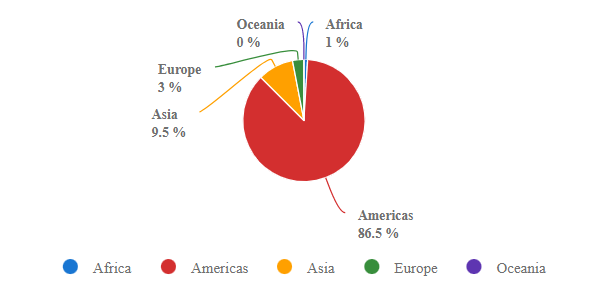
\includegraphics[width=12cm]{image/img1.png}
    \end{center}
    \legend{Fonte: \cite{FAOSTAT2022}}
\end{figure}


Neste mesmo período o Brasil deixou o posto de segundo lugar para ser o maior produtor de soja - na safra de 2001/2002, a produção brasileira era aproximadamente 52 milhões de toneladas, nesta mesma safra o EUA era aproximadamente 75 milhões de toneladas, agora na safra 2021/2022 o Brasil alcançou perto de 122 milhões toneladas, superior ao EUA que entorno de 120,7 milhões de toneladas, conforme dados da \cite{conab2022}.

\begin{figure}
  \caption{\label{imagen2}Produção de Soja por ano no Brasil de 1994 a 2020}
    \begin{center}
      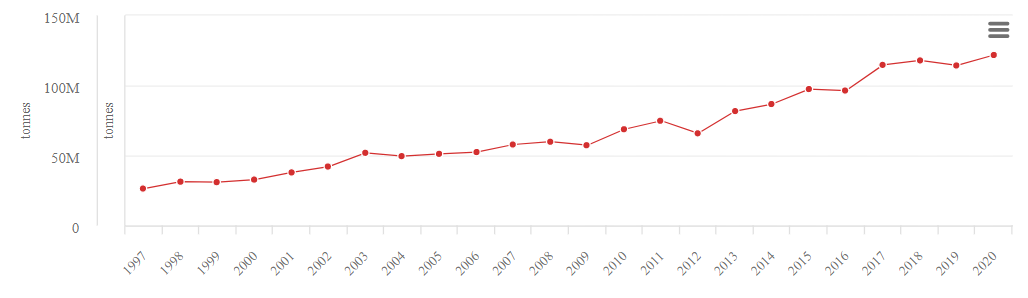
\includegraphics[scale = 0.7]{image/img2.png}
    \end{center}
    \legend{Fonte: \cite{FAOSTAT2022}}
\end{figure}


Diante do exposto deste trabalho, pretende à aplicação de modelos \textbf{ARIMA} (Autorregressivos Integrados de Médias Móveis) nos índices de preços da \textit{commodities} soja com a finalidade de compreender o comportamento da 
comercialização deste produto.


% ----------------------------------------------------------
% Capitulo de textual
% ----------------------------------------------------------
\chapter{Séries Temporais}
  
Qualquer conjunto de observações ordenadas no tempo, é uma série temporal. Por exemplos:

\begin{itemize}
  \item[\textit{i)}] temperaturas médias diárias de uma cidade;
  \item[\textit{ii)}] vendas mensais de uma empresa;
  \item[\textit{iii)}] valores de fechamento diários da IBOVESPA;
  \item[\textit{iv)}] preços diários de \textit{commodities};
  \item[\textit{v)}] valores mensais do IPCA (Índice Nacional de Preços ao Consumidor Amplo).
\end{itemize}

As séries temporais podem ser tanto discreta quanto contínua, ou seja, discreta é o 
intervalo entre as observações pertecentes a um conjunto discreto, e contínua é o 
intervalo entre as observações pertecentes a um conjunto contínuo. Observa-se que 
quando dizemos que uma série é discreta, estamos fazendo referência ao tempo entre as 
observações e não a escala da variável.

Além disso, temos dois enfoques usados na análise de séries temporais. O objetivo de ambos é construir modelos para as séries. No primeiro enfoque é feita análise no \textit{domínio temporal} e os modelos sugeridos são \textit{modelos paramétricos} (números de parâmetros finitos), o segundo é conduzido no \textit{domínio de frequências} e os propostos são 
\textit{modelos não-paramétricos} \cite{morettin2006analise}. O modelo utilizado neste 
estudo, \textbf{ARIMA} é um modelo paramétrico.




  \section{Processos Estocásticos}
  
Podemos definir um processo estocástico como um conjunto cronológico de observações de um determinado fenômeno de forma que o seu comportamento pode ser descrito por uma ou mais distribuições de probabilidade. Conforme \cite{morettin2006analise},


\begin{definition}

Seja $T$ um conjunto arbitrário, um processo estocástico é uma família de variáveis aleatórias 
$\left\{Z(t),\ t \in T \right\}$, tal que, $\forall t \in T$,  $Z(t)$ é uma variável aleatória.

\end{definition}
  
\begin{figure}
  \caption{\label{img4}Família de trajetórias de processos estocásticos.}
    \begin{center}
      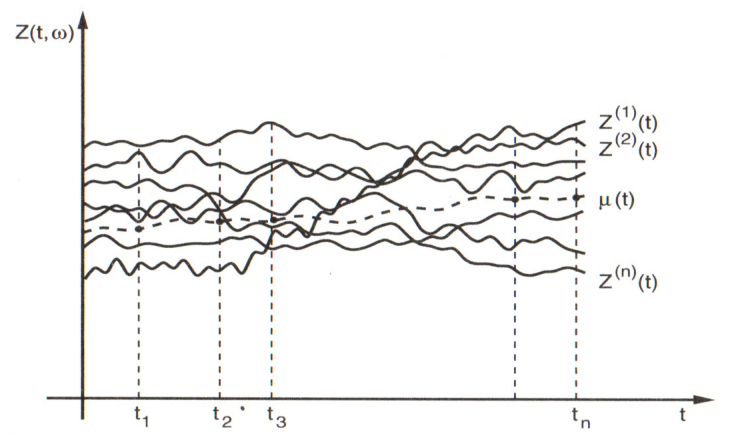
\includegraphics[scale = 0.9]{image/img4.png}
    \end{center}
    \legend{Fonte: \cite{morettin2006analise}}
\end{figure}

Neste caso, um processo estocástico é uma família de variáveis aleatórias, definidas num mesmo espaço de probabilidade $(\Omega, \mathcal{A}, \mathcal{P})$, tendo o conjunto $T$, normalmente tomado como conjunto dos inteiros $\mathbb{Z} = \left\{0,\pm 1, \pm 2, \ldots \right\}$ ou conjunto dos reais $\mathbb{R}$.

A Figura \ref{img3} ilustra uma interpretação de um processo estocástico, ou seja, para $t \in T,\ Z(t)$ é uma variável aleatória definida em $\Omega$, e $Z(t)$ é uma função de dois argumentos $Z(t, \omega)$, $t \in T$, $\omega \in \Omega$. Na figura, cada $t \in T$, temos uma v.a. $Z(t, \omega)$, com uma distribuição de probabilidade, é possível que a função densidade de probabilidade (fdp) no instante $t_1$ seja distinta da fdp no instante $t_2$, entre os instante $t_1$ e $t_2$ quaisquer, mas usualmente é aquela em que a fdp de $Z(t, \omega)$ é a mesma, $\forall t \in T$.



\begin{figure}
  \caption{\label{img3}Um processo estocástico interpretado como uma família de variáveis.}
    \begin{center}
      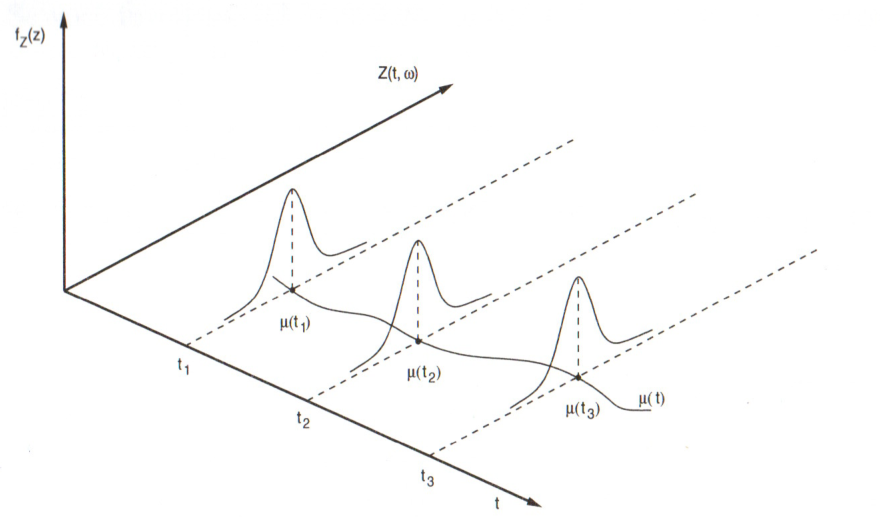
\includegraphics[scale = 0.9]{image/img3.png}
    \end{center}
    \legend{Fonte: \cite{morettin2006analise}}
\end{figure}

  
  \section{Modelos ARIMA}
  
Segundo \cite{martins2014comparison} a metodologia Box-Jenkins possibilita detectar distintos modelos ARIMA e entre eles: o modelo Autoregressivo de ordem p (AR), o modelo de Médias Móveis de ordem q (MA), o modelo Autoregressivo de Médias Móveis de ordem p e q (ARMA), o modelo Autoregressivo Integrado de Médias Móveis, de ordem p, q contendo diferença d (ARIMA) que, apresenta como o principal caso contido nessa técnica. Segundo Ramser et al. (2015), eles apresentam conduta estacionária nos modelos AR(p) e MA(p), assim como a junção destes, o modelo ARMA(p,q).

O modelo ARIMA (p,d,q) é o efeito do uso de diferenciação na séries onde a média é variante,
transformando-os estacionárias. Os modelos estacionários e os não estacionários, diferenciam-se
pela quantidade de diferenças necessárias para estabilizar a série, simbolizado pela letra d \cite{martins2014comparison}.

Ao ajustar um modelo ARIMA a um conjunto de dados de séries temporais, o procedimento a seguir fornece uma abordagem geral útil \cite{hyndman2018forecasting}.

\begin{itemize}
  \item Plote os dados e identifique quaisquer observações incomuns;
  \item Se necessário, transforme os dados (usando uma transformação Box-Cox) para estabilizar a variação;
  \item Se os dados não forem estacionários, tome as primeiras diferenças dos dados até que os dados sejam estacionários;
  \item Examine o ACF/PACF: É um ARIMA(p,d,0) ou ARIMA(0,d,q) modelo apropriado?;
  \item Experimente o(s) modelo(s) escolhido(s) e use o AICc para procurar um modelo melhor;
  \item Verifique os resíduos do modelo escolhido plotando o ACF dos resíduos e fazendo um teste portmanteau dos resíduos. Se eles não se parecerem com ruído branco, tente um modelo modificado;
  \item Quando os resíduos parecerem ruído branco, calcule as previsões.
\end{itemize}

Este processo é usado pela função "auto.arima" do pacote "forecast" Software R. Resumido na Figura \ref{img13}.

\begin{figure}
  \caption{\label{img13}Processo geral de previsão usando um modelo ARIMA.}
    \begin{center}
      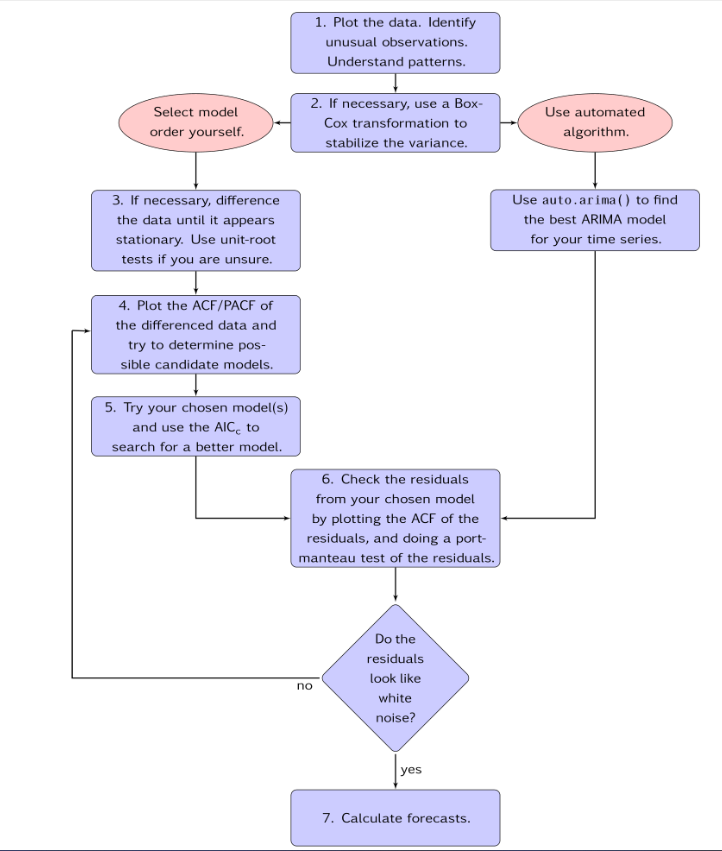
\includegraphics[width=12cm]{image/img5.png}
    \end{center}
    \legend{Fonte: \cite{hyndman2018forecasting}}
\end{figure}

\chapter{Metodologia}

Para obtenção das análises estatísticas dos dados, fez-se o uso do \textit{software} \textbf{R} (versão 4.2.1). Com posse dos dados, foi realizada uma análise inicial dos dados para identificar o comportamento da série temporal e analisar suas características  quanto tendência, sazonalidade, aleatoriedade e existência de ruídos.


O índice de Preços da \textit{commodities} Soja foi adquirido no site do CEPEA (Centro de Estudos Avançados em Economia Aplicada), com intervalo de outubro de 1997 até outubro de 2022.



\chapter{Resultados e Discussões}




A Tabela \ref{tab1} apresenta as principais medidas descritivas obtidas a partir da série mensal 
condizente ao indicador de preços em reais da soja (reais por saca de 60 kg) compreendido 
no período de outubro de 1997 a outubro de 2022, proporcionanddo uma visão panorâmica do comportamento da série em estudo.
Com isso é possível observar-se que ao longo de 25 anos o menor valor do preço foi de R\$ 13,87 (agosto de 1998) e o maior valor R\$ 195,85 (março de 2022), além de algumas medidas que quantificam a dispersão dos dados, tais como o desvio-padrão $sd = 40,91$ e o coeficiente de variação $CV = 69,77$.

\begin{knitrout}
\definecolor{shadecolor}{rgb}{0.969, 0.969, 0.969}\color{fgcolor}\begin{table}[!h]

\caption{\label{tab:script3}Estística Descritiva \label{tab1}}
\centering
\begin{tabular}[t]{rrrrrr}
\toprule
Min. & 1st Qu. & Median & Mean & 3rd Qu. & Max.\\
\midrule
\cellcolor{gray!6}{13.87} & \cellcolor{gray!6}{31.34} & \cellcolor{gray!6}{46.8} & \cellcolor{gray!6}{58.63} & \cellcolor{gray!6}{72.91} & \cellcolor{gray!6}{195.8}\\
\bottomrule
\end{tabular}
\end{table}

\end{knitrout}



A Figura \ref{fig1} apresenta a série original do indicador de preço médio mensal em reais da soja no intervalo de outubro de 1997 a outubro de 2022. Observa-se que o comportamento da série apresenta uma tendência não uniforme em seus preços.

\begin{knitrout}
\definecolor{shadecolor}{rgb}{0.969, 0.969, 0.969}\color{fgcolor}\begin{figure}[H]
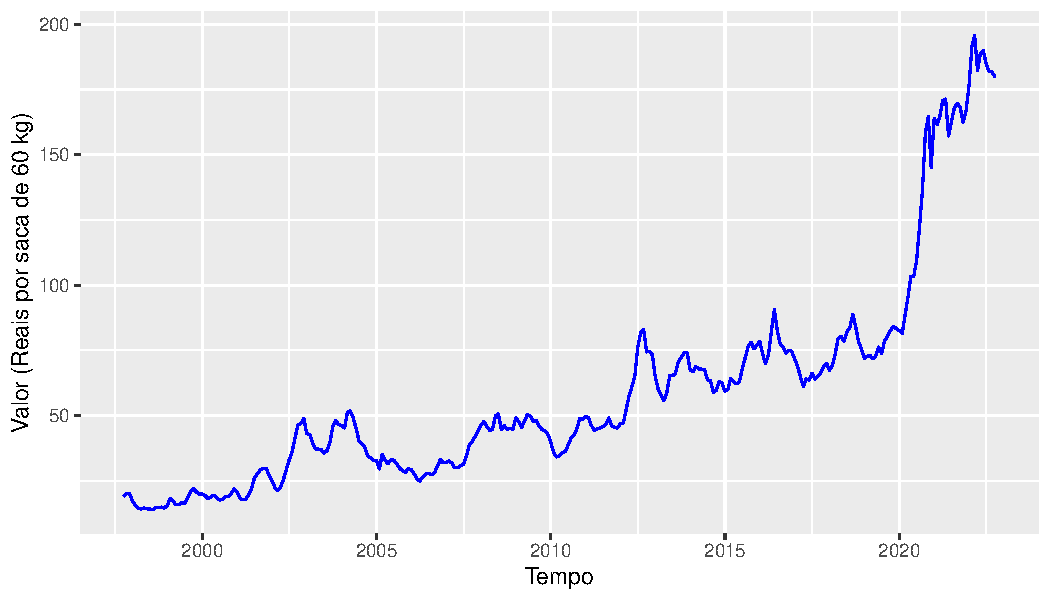
\includegraphics[width=\maxwidth]{figure/script1-1} \caption[Indicador de preço da soja no período de outubro de 1997 até outubro de 2022 \label{fig1}]{Indicador de preço da soja no período de outubro de 1997 até outubro de 2022 \label{fig1}}\label{fig:script1}
\end{figure}

\end{knitrout}

Pode-se observar na apresentação da Figura \ref{fig2} a decomposição da série em componentes: série original, parte aleatória, sazonalidade e tendência. Em vista disso, constata-se que a série oscila em torno de uma valor médio do preço da soja e com um padrão recorrente bem definido, o que deixa implícito a presença de sazonalidade aditiva e a existência de tendência nos dados.


\begin{knitrout}
\definecolor{shadecolor}{rgb}{0.969, 0.969, 0.969}\color{fgcolor}\begin{figure}
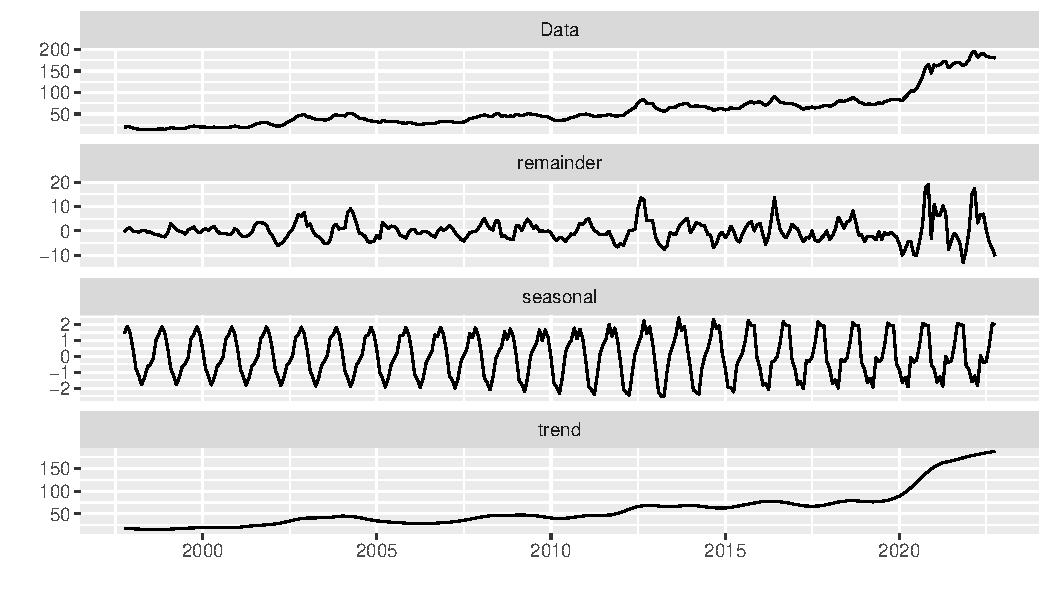
\includegraphics[width=\maxwidth]{figure/script2-1} \caption[Decomposição da série de preço da soja]{Decomposição da série de preço da soja.\label{fig2}}\label{fig:script2}
\end{figure}

\end{knitrout}

Na Figura \ref{fig4}, é possível verificar o comportamento anual do preço médio mensal, composto de 301 observações, onde pode-se observar que os preços mais altos concentram nos meses de maio e junho e com mais variabilidade dos preços. Mas os preços médio em meses apresentaram comportamentos de variação similares entre si. Pode-se notar que todos os meses apresentaram no mínimo um valor atípico (outlier).

\begin{knitrout}
\definecolor{shadecolor}{rgb}{0.969, 0.969, 0.969}\color{fgcolor}\begin{figure}[H]
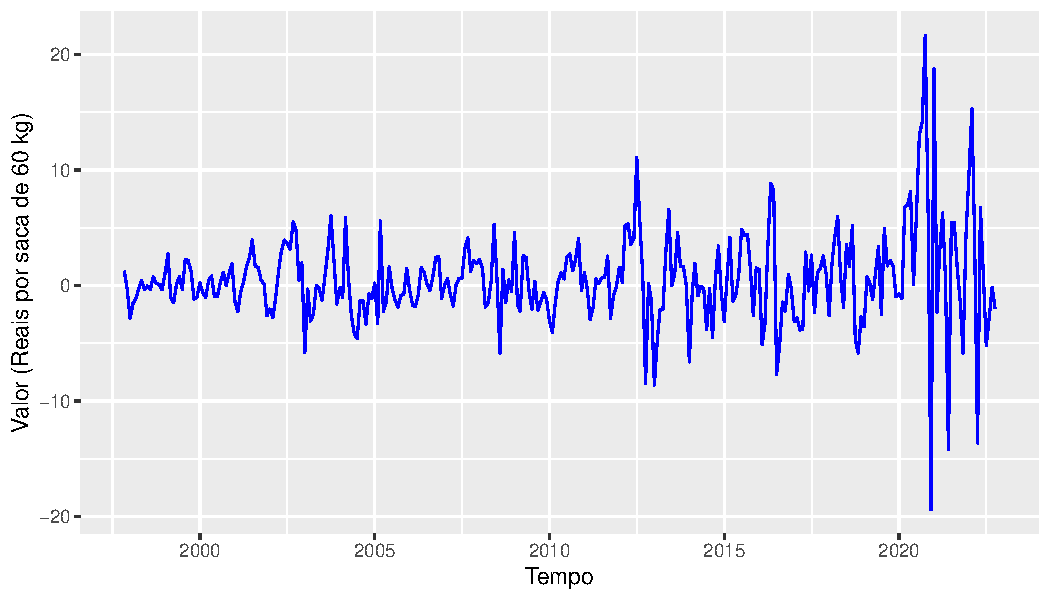
\includegraphics[width=\maxwidth]{figure/script5-1} \caption[ Gráfico de Boxplot, da série distribúida entre os meses (período de 10/1997 a 10/2022)]{ Gráfico de Boxplot, da série distribúida entre os meses (período de 10/1997 a 10/2022).\label{fig4}}\label{fig:script5}
\end{figure}

\end{knitrout}


As funções de autocorrelação (ACF) e autocorrelação parcial (PACF) da série, representadas na Figura \ref{fig3}, nota-se que ela decresce rapidamente, indicando a estacionariedade da série 


\begin{knitrout}
\definecolor{shadecolor}{rgb}{0.969, 0.969, 0.969}\color{fgcolor}\begin{figure}
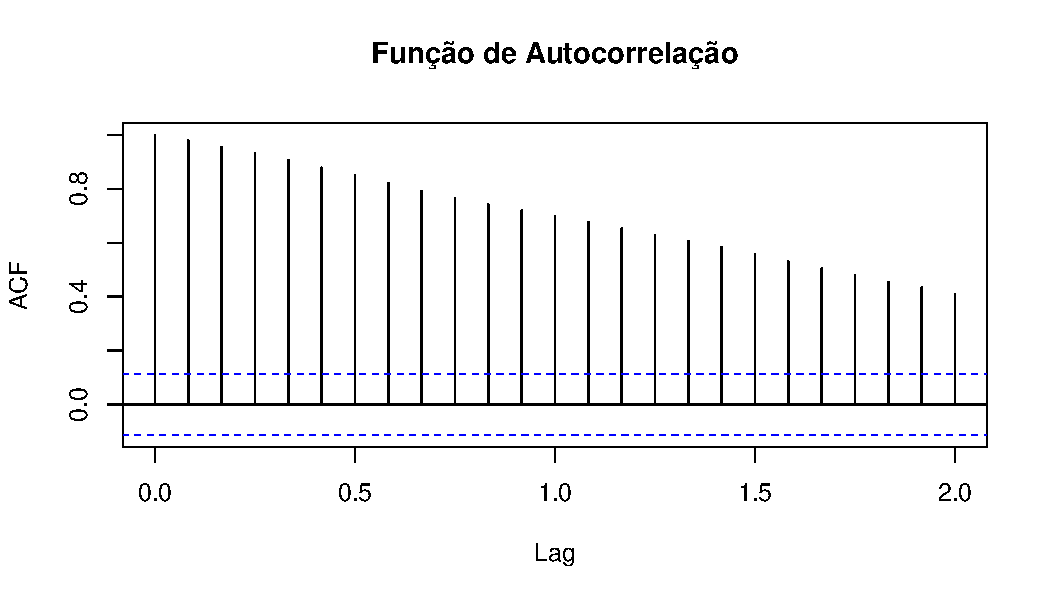
\includegraphics[width=\maxwidth]{figure/script4-1} \caption[Correlograma da série]{Correlograma da série.\label{fig3}}\label{fig:script4}
\end{figure}

\end{knitrout}


Após ser aplicada a diferença, foi plotado novamente as funções para confirmar a eliminação da componente sazonal, e identificar as ordens de possíveis modelos \textbf{ARIMA} para a série. A Figura \ref{fig4}c, obersa que a ao aplicar a diferenciação, a série aparenta está estacionária na média, mas a variância é crescente ao longo do tempo. Como um dos pressupostos da teoria Box \& Jenkins é que a série seja também estacionaária na variância. Para tal, aplicaremos o logaritmo na série em questão. A Figura \ref{fig4}d nos mostra que temos a série estacionária na média e na variância.

\begin{knitrout}
\definecolor{shadecolor}{rgb}{0.969, 0.969, 0.969}\color{fgcolor}\begin{figure}
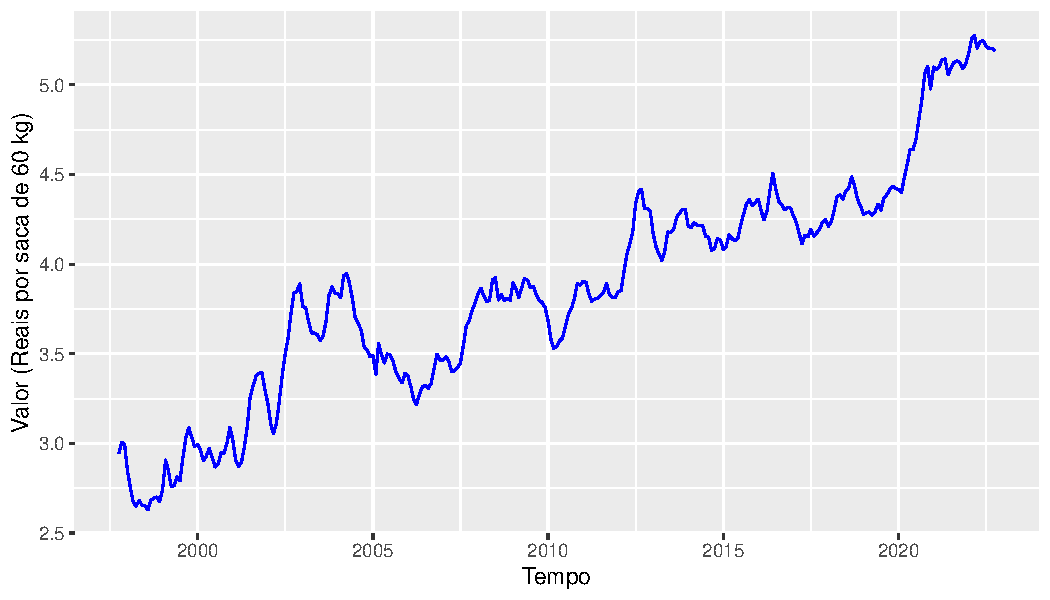
\includegraphics[width=\maxwidth]{figure/script6-1} \caption[Gráficos]{Gráficos: a) Função de Autocorrelação da série logaritma diferenciada; b) Função de Autocorrelaçaõ Parcial da série logaritma diferenciada; c) Comportamento da variação da série diferenciada; e d) Logaritmo da diferenciação da série, para estabilizar a variância.\label{fig4}}\label{fig:script6}
\end{figure}

\end{knitrout}


Analisando os correlogramas anteriores, alguns coeficientes se mostraram não significativosfica claro que aplicando a diferenciação, a série torna-se estacionária. Para uma melhor verificação da função de autocorrelação e autocorrelação parical, aplicaremos testes para verificar a estacionariedade da série, tais: o \textit{teste de Dickey-Fuller Aumentado}, \textit{Raiz Unitária}; teste de \textit{Phillips-Perron}; teste de KPSS (Kwiatkowski, Philips, Schimidt e Shin). 

\begin{knitrout}
\definecolor{shadecolor}{rgb}{0.969, 0.969, 0.969}\color{fgcolor}\begin{kframe}
\begin{alltt}
\hlcom{# Teste ADF.}
\hlkwd{adf.test}\hlstd{(Soja.log.dif1)}
\end{alltt}
\begin{verbatim}
## 
## 	Augmented Dickey-Fuller Test
## 
## data:  Soja.log.dif1
## Dickey-Fuller = -7.6002, Lag order = 6, p-value = 0.01
## alternative hypothesis: stationary
\end{verbatim}
\begin{alltt}
\hlcom{# Teste de Phillips-Perron.}
\hlkwd{pp.test}\hlstd{(Soja.log.dif1)}
\end{alltt}
\begin{verbatim}
## 
## 	Phillips-Perron Unit Root Test
## 
## data:  Soja.log.dif1
## Dickey-Fuller Z(alpha) = -186.81, Truncation lag parameter = 5, p-value
## = 0.01
## alternative hypothesis: stationary
\end{verbatim}
\begin{alltt}
\hlcom{# Teste KPSS.}
\hlkwd{kpss.test}\hlstd{(Soja.log.dif1,} \hlkwc{null} \hlstd{=} \hlstr{"Level"}\hlstd{)}
\end{alltt}
\begin{verbatim}
## 
## 	KPSS Test for Level Stationarity
## 
## data:  Soja.log.dif1
## KPSS Level = 0.050398, Truncation lag parameter = 5, p-value = 0.1
\end{verbatim}
\end{kframe}
\end{knitrout}

Anunciando nossa hipótese, a regra de decisão da rejeição ou não da hipótese nula ($H_0$) é: se o \textit{p-valor} é menor que o valor significativo, então rejeita-se $H_0$. Caso contrário, não rejeita-se $H_0$. Com isso, podemos verificar pelo teste que o \textit{p-valor} é menor que o valor significativo de 5\%. Apenas no teste de KPSS o anunciado das hipóteses são inversas, neste caso todos os testes indicam que a série é estacionária. Após a identificação das ordens de diferenciação sequêncial e sazonal, tem-se um modelo com a seguinte característica \textbf{ARIMA($p,1,q$)($P,1,Q$)}.

\begin{equation*}
\begin{split}
H_0 & : \text{A série não é estacionária.} \\
H_1 & : \text{A série é estacionária.}
\end{split}
\end{equation*}


\begin{knitrout}
\definecolor{shadecolor}{rgb}{0.969, 0.969, 0.969}\color{fgcolor}\begin{kframe}
\begin{alltt}
\hlcom{# Teste ADF.}
\hlkwd{adf.test}\hlstd{(Soja.log.dif1)}
\end{alltt}
\begin{verbatim}
## 
## 	Augmented Dickey-Fuller Test
## 
## data:  Soja.log.dif1
## Dickey-Fuller = -7.6002, Lag order = 6, p-value = 0.01
## alternative hypothesis: stationary
\end{verbatim}
\begin{alltt}
\hlcom{# Teste de Phillips-Perron.}
\hlkwd{pp.test}\hlstd{(Soja.log.dif1)}
\end{alltt}
\begin{verbatim}
## 
## 	Phillips-Perron Unit Root Test
## 
## data:  Soja.log.dif1
## Dickey-Fuller Z(alpha) = -186.81, Truncation lag parameter = 5, p-value
## = 0.01
## alternative hypothesis: stationary
\end{verbatim}
\begin{alltt}
\hlcom{# Teste KPSS.}
\hlkwd{kpss.test}\hlstd{(Soja.log.dif1,} \hlkwc{null} \hlstd{=} \hlstr{"Level"}\hlstd{)}
\end{alltt}
\begin{verbatim}
## 
## 	KPSS Test for Level Stationarity
## 
## data:  Soja.log.dif1
## KPSS Level = 0.050398, Truncation lag parameter = 5, p-value = 0.1
\end{verbatim}
\end{kframe}
\end{knitrout}


Como é demasiado o serviço para selecionar valores apropriado para cada um desses três parâmetros, a função "forecast::auto.arima()", faz automaticamente.

\begin{knitrout}
\definecolor{shadecolor}{rgb}{0.969, 0.969, 0.969}\color{fgcolor}\begin{kframe}
\begin{alltt}
\hlcom{# Estimativa do modelo ARIMA.}
\hlstd{mod.arima} \hlkwb{<-} \hlkwd{auto.arima}\hlstd{(Soja_log)}
\hlkwd{summary}\hlstd{(mod.arima)}
\end{alltt}
\begin{verbatim}
## Series: Soja_log 
## ARIMA(1,1,0)(2,0,0)[12] with drift 
## 
## Coefficients:
##          ar1    sar1     sar2   drift
##       0.3645  0.0334  -0.1166  0.0076
## s.e.  0.0539  0.0585   0.0615  0.0047
## 
## sigma^2 = 0.003132:  log likelihood = 440.99
## AIC=-871.97   AICc=-871.77   BIC=-853.45
## 
## Training set error measures:
##                         ME       RMSE        MAE         MPE     MAPE      MASE
## Training set -4.198801e-05 0.05550114 0.04369263 -0.01376519 1.172031 0.2158349
##                    ACF1
## Training set 0.02564065
\end{verbatim}
\end{kframe}
\end{knitrout}

O modelo resultante é um ARIMA(1,1,0)(2,0,0), o que corresponde a uma combinação a uma série com um grau de diferenciação ($p = 1$) aplicada em um modelo AR(1) e em um MA(0). Antes de fazer a previsão, faremos uma análise de resíduos. Podemos verificar na Figura \ref{fig11} que o gráfico ACF dos resíduos do modelo \textbf{ARIMA}(1,1,0)(2,0,0) mostra que todas as autocorrelações estão dentro dos limites, indicando que os resíduos estão se comportando como ruído branco. E o teste de Ljung-Box retorna um grande p-valor (maior do que o valor significativo de 5\%), sugerindo também que os resíduos são ruído branco. 

\begin{knitrout}
\definecolor{shadecolor}{rgb}{0.969, 0.969, 0.969}\color{fgcolor}\begin{figure}
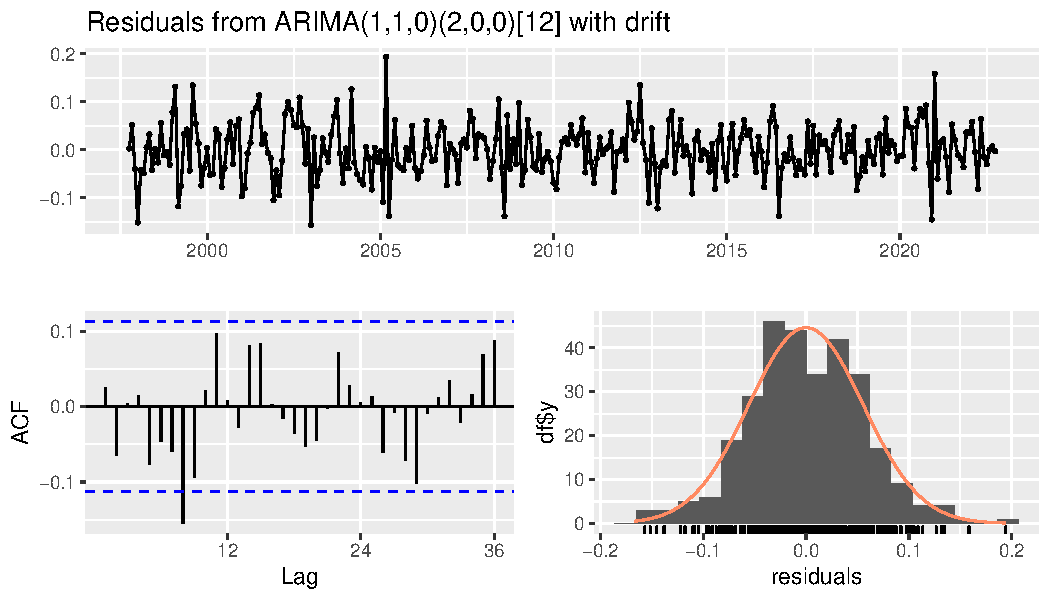
\includegraphics[width=\maxwidth]{figure/script11-1} \caption[Gráficos de resíduos para o modelo ARIMA(1,1,0)(2,0,0)]{Gráficos de resíduos para o modelo ARIMA(1,1,0)(2,0,0).\label{fig11}}\label{fig:script11}
\end{figure}

\begin{kframe}\begin{verbatim}
## 
## 	Ljung-Box test
## 
## data:  Residuals from ARIMA(1,1,0)(2,0,0)[12] with drift
## Q* = 26.983, df = 21, p-value = 0.1714
## 
## Model df: 3.   Total lags used: 24
\end{verbatim}
\end{kframe}
\end{knitrout}


Agora faremos a previsão da série, apresentado na Figura \ref{fig12} seguinte.

\begin{knitrout}
\definecolor{shadecolor}{rgb}{0.969, 0.969, 0.969}\color{fgcolor}\begin{figure}
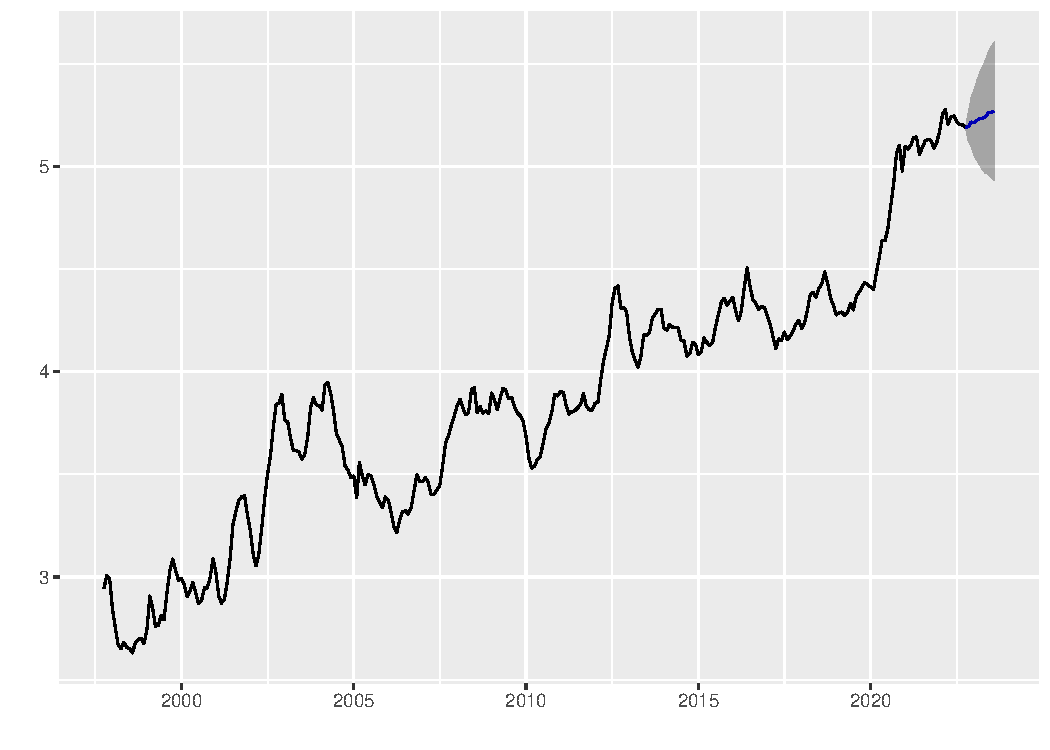
\includegraphics[width=\maxwidth]{figure/script12-1} \caption[Previsão para o indíce de preço da soja]{Previsão para o indíce de preço da soja.\label{fig12}}\label{fig:script12}
\end{figure}

\end{knitrout}





\chapter{Considerações Finais}

O presente trabalho teve como objetivo estudar o comportamento do preço da Soja no Brasil, e testar a metodologia Box \& Jenkins para previsão. Para isso foi utilizado uma função do pacote "forecast" do Software R para obter o modelo ideal para série, função está que é automatizada que reduz o número de combinações de modelos possíveis adequados. O modelo destacado foi o ARIMA(1,1,0)(2,0,0). De posse deste modelo é possível inferir o preço futuro da saca de 60kg da soja comercializada no Brasil, possibilitando assim melhor planejamento da compra, venda e produção desse grão.

Algumas lmiitações podem ser revistas em estudos futuros, como: (a) relacionar outras técnicas de previsão; (b) relacionar eventos pontuais em cada ano e identificar o quanto influência no preço da soja. Este estudo pode contribuir para pesquisas acadêmicas de métodos quantitativos de previsão e para entender os valores futuros do produto para prentensão de aumentar seus lucros. 



% ----------------------------------------------------------
\bibliography{abntex2-modelo-references}

% ----------------------------------------------------------
% Glossário
% ----------------------------------------------------------
%
% Consulte o manual da classe abntex2 para orientações sobre o glossário.
%
%\glossary

% ----------------------------------------------------------
% Apêndices
% ----------------------------------------------------------

% ---
% Inicia os apêndices
% ---

% Tirar os restantes das páginas não textuais.



\begin{apendicesenv}

% Imprime uma página indicando o início dos apêndices
\partapendices

% ----------------------------------------------------------
\chapter{SCRIPT R}
% ----------------------------------------------------------

\begin{knitrout}\tiny
\definecolor{shadecolor}{rgb}{0.969, 0.969, 0.969}\color{fgcolor}\begin{kframe}
\begin{alltt}
\hlkwd{library}\hlstd{(forecast)}   \hlcom{# Ferramentas para exibir e analisar previsões de séries temporais univariadas.}
\hlkwd{library}\hlstd{(timeSeries)} \hlcom{# Ferramentas para séries temporais financeiras.}
\hlkwd{library}\hlstd{(urca)}       \hlcom{# Testes de raiz unitária e de cointegração.}
\hlkwd{library}\hlstd{(randtests)}  \hlcom{# Testes de aleatoriedade não paramétricos para sequências numéricas.}
\hlkwd{library}\hlstd{(tseries)}    \hlcom{# Análise de séries temporais e finanças computacionais.}
\hlkwd{library}\hlstd{(stats)}      \hlcom{# Funções para cálculos estatísticos e geração de números aleatórios.}
\hlkwd{library}\hlstd{(readxl)}     \hlcom{# Importe arquivos Excel para R.}
\hlkwd{library}\hlstd{(tidyverse)}  \hlcom{# Conjunto de pacotes que funcionam em harmonia para data analysis.}
\hlkwd{library}\hlstd{(ggfortify)}  \hlcom{# Ferramentas de plotagem unificadas.}
\hlkwd{library}\hlstd{(magrittr)}   \hlcom{# Fornece o encadeamento de comandos, pipeline (%>%).}
\hlkwd{library}\hlstd{(kableExtra)} \hlcom{# Gerador de tabelas.}

\hlstd{soja} \hlkwb{<-} \hlkwd{read_xls}\hlstd{(}\hlstr{"...dataset/soja.xls"}\hlstd{)} \hlcom{# Importar o conjunto de dados.}

\hlstd{soja} \hlkwb{<-} \hlkwd{ts}\hlstd{(soja}\hlopt{$}\hlstd{Preço,} \hlkwc{start} \hlstd{=} \hlkwd{c}\hlstd{(}\hlnum{1997}\hlstd{,}\hlnum{10}\hlstd{),} \hlkwc{frequency} \hlstd{=} \hlnum{12}\hlstd{)} \hlcom{# Criar o objeto de série temporal.}

\hlkwd{class}\hlstd{(soja)} \hlcom{# Retornar os valores do atributo de classe de um objeto.}
\hlkwd{as.ts}\hlstd{(soja)} \hlcom{# Testar se o objeto é um série temporal.}

\hlcom{### Informações descritiva da série (resumo).}
\hlkwd{summary}\hlstd{(soja)}

\hlcom{### Plotagem da série original.}
\hlkwd{autoplot}\hlstd{(soja,} \hlkwc{xlab} \hlstd{=} \hlstr{"Tempo"}\hlstd{,} \hlkwc{ylab} \hlstd{=} \hlstr{"Valor (Reais por saca de 60 kg)"}\hlstd{,} \hlkwc{ts.colour} \hlstd{=} \hlstr{'blue'}\hlstd{)}

\hlcom{### Decomposição da série e plotagem.}
\hlstd{soja} \hlopt
  \hlkwd{stl}\hlstd{(,} \hlkwc{s.window} \hlstd{=} \hlstr{"periodic"}\hlstd{)} \hlopt
    \hlkwd{autoplot}\hlstd{(,} \hlkwc{ts.colour} \hlstd{=} \hlstr{"blue"}\hlstd{)}

\hlcom{### }
\end{alltt}
\end{kframe}
\end{knitrout}





\end{apendicesenv}
% ---


\end{document}
